
\begin{frame}{Contents}
   \begin{itemize}
       \item[\textcolor{red}{$\checkmark$}] Chisel の導入
       \item[\textcolor{red}{$\rhd$}] Pros. \& Cons.
       \item ChiselImProc の説明
       \item Vivado HLS との比較
   \end{itemize} 
\end{frame}



\begin{frame}{Pros. \& Cons.}
            \begin{block}{Pros.}
                \begin{itemize}
                    \item OOP の強みは大体使える。
                    \item 型パラメータを利用できる。
                    \item 再利用性は高い。
                    \item 出力されたvファイルと元のScalaのコードの対応が見やすい。
                    
                \end{itemize}
            \end{block}
            \begin{block}{Cons.}
                \begin{itemize}
                    \item クロックは常に意識しないと厳しい。
                    \item AXI はchisel3だと結局ない(?)
                    \item vファイルがやたら重い。
                    \item XRESETには対応していない。
                \end{itemize}
            \end{block}
    
\end{frame}

\begin{frame}[fragile]{AXI Stream}
    \begin{itemize}
        \item 型パラメータを利用できる。
        \item 上限境界 (<:) なども利用できる。
        \begin{lstlisting}[caption={"AXI Stream Interface"}]
class AXIStreamIF[T <: Data](gen: T) 
        extends ReadyValidIO[T](gen) {
    val user = Output (Bool())
    val last = Output (Bool())

    override def cloneType: this.type 
        = new AXIStreamIF(gen).asInstanceOf[this.type]
}

object AXIStreamMasterIF {
    def apply [T <: Data] (gen: T): AXIStreamIF[T] 
        = new AXIStreamIF[T] (gen)
}

object AXIStreamSlaveIF {
    def apply [T <: Data] (gen: T): AXIStreamIF[T] 
        = Flipped (new AXIStreamIF[T] (gen))
}            
        \end{lstlisting}
        
        \item Data 型はChisel のすべてのデータのsupertype
    \end{itemize}
    
\end{frame}




\begin{frame}{Data Types Overview}
    \begin{figure}[h]
        \centering
        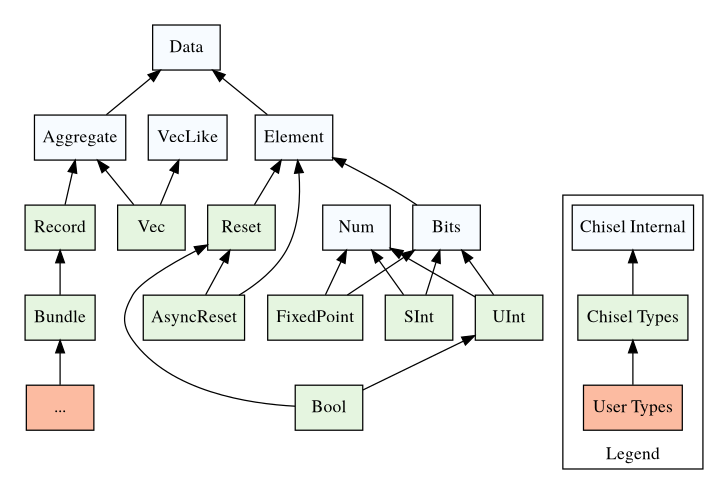
\includegraphics[width=\textwidth]{./figures/type_hierarchy.png}
    \end{figure}
\end{frame}



\begin{frame}[fragile]{AXI Streamを用いたモジュール}
    \begin{lstlisting}
class FifoAXIStreamDIO[T <: Data, U <: Data] (
    private val genEnq: T,
    private val genDeq: U
) extends Bundle {
    val enq = AXIStreamSlaveIF(genEnq)
    val deq = AXIStreamMasterIF(genDeq)
}

class FifoAXIStreamIO[T <: Data] (private val gen: T)
        extends FifoAXIStreamDIO(gen, gen) {
}

abstract class FifoAXIS[T <: Data] (gen: T, depth: Int)
        extends Module {
    val io = IO (new FifoAXIStreamIO[T] (gen))
    assert (depth > 0, 
        "Number of buffer elements needs to be larger than 0")
}
    \end{lstlisting}
    
    ※ enq と deq は Chiselと僕のコードで逆。
\end{frame}

\begin{frame}[fragile]{積和モジュール}

\begin{itemize}
    \item 8bit で3x3は遅延しない(1クロックで動作できる)
    \item 8bit で5x5は遅延する(1クロックで動作できない)
    \item 16bit で3x3は遅延?
\begin{lstlisting}
class MulAdd (dataWidth: Int, num: Int) extends Module {
    val io = IO(new Bundle {
        val a = Input (Vec(num, UInt(dataWidth.W)))
        val b = Input (Vec(num, UInt(dataWidth.W)))
        val output = Output (UInt ((2*dataWidth).W))
    })

    var i = 0
    var tmp = 0.U((2*dataWidth).W)
    val step = 3                // 8bit で3x3は遅延しない
    for (i <- 0 until num by step) {
        var intmp = 0.U((2*dataWidth).W)
        for (j <- 0 until step) {
            intmp += io.a(i+j) * io.b (i+j)
        }
        tmp += intmp
    }
    io.output := tmp    
}
\end{lstlisting}
\end{itemize}
    
\end{frame}



\begin{frame}[fragile]{Verilogファイル生成}
    \begin{itemize}
        \begin{lstlisting}[language={Verilog}, basicstyle={\tiny}]
module MulAdd(
  input  [7:0]  io_b_0,
  input  [7:0]  io_b_1,
  input  [7:0]  io_b_2,
  input  [7:0]  io_b_3,
  input  [7:0]  io_b_4,
  input  [7:0]  io_b_5,
  input  [7:0]  io_b_6,
  input  [7:0]  io_b_7,
  input  [7:0]  io_b_8,
  output [15:0] io_output
);
  wire [15:0] _T = 8'h1 * io_b_0; // @[ChiselImProc.scala 32:32]
  wire [16:0] _T_1 = {{1'd0}, _T}; // @[ChiselImProc.scala 32:19]
  wire [15:0] _T_3 = 8'h2 * io_b_1; // @[ChiselImProc.scala 32:32]
  wire [15:0] _T_5 = _T_1[15:0] + _T_3; // @[ChiselImProc.scala 32:19]
  wire [15:0] _T_6 = 8'h1 * io_b_2; // @[ChiselImProc.scala 32:32]
  wire [15:0] _T_8 = _T_5 + _T_6; // @[ChiselImProc.scala 32:19]
  wire [16:0] _T_9 = {{1'd0}, _T_8}; // @[ChiselImProc.scala 34:13]
  wire [15:0] _T_11 = 8'h2 * io_b_3; // @[ChiselImProc.scala 32:32]
  wire [16:0] _T_12 = {{1'd0}, _T_11}; // @[ChiselImProc.scala 32:19]
  wire [15:0] _T_14 = 8'h4 * io_b_4; // @[ChiselImProc.scala 32:32]
  wire [15:0] _T_16 = _T_12[15:0] + _T_14; // @[ChiselImProc.scala 32:19]
  wire [15:0] _T_17 = 8'h2 * io_b_5; // @[ChiselImProc.scala 32:32]
  wire [15:0] _T_19 = _T_16 + _T_17; // @[ChiselImProc.scala 32:19]
  wire [15:0] _T_21 = _T_9[15:0] + _T_19; // @[ChiselImProc.scala 34:13]
  wire [15:0] _T_22 = 8'h1 * io_b_6; // @[ChiselImProc.scala 32:32]
  wire [16:0] _T_23 = {{1'd0}, _T_22}; // @[ChiselImProc.scala 32:19]
  wire [15:0] _T_25 = 8'h2 * io_b_7; // @[ChiselImProc.scala 32:32]
  wire [15:0] _T_27 = _T_23[15:0] + _T_25; // @[ChiselImProc.scala 32:19]
  wire [15:0] _T_28 = 8'h1 * io_b_8; // @[ChiselImProc.scala 32:32]
  wire [15:0] _T_30 = _T_27 + _T_28; // @[ChiselImProc.scala 32:19]
  assign io_output = _T_21 + _T_30; // @[ChiselImProc.scala 36:15]
endmodule
        \end{lstlisting}
    \end{itemize}
    
\end{frame}



\begin{frame}{Verilogファイル生成}
\begin{itemize}
    \item IO, Register, Wire は変数名がそのまま使われる。
    \item フィールド名は\_で分けられる。
    \item 計算途中のデータなどは\_T\_番号で名付けられる。
    \item コメントで元のScalaのどこの部分と対応しているか明記される。
    \item 使われていないWireやRegisterなどは消される。
    \item 出力のvファイルを分割できない。\\
        -fsm, --split-modulesオプションをつければ分けれそうだが分けれない。
\end{itemize}
    
\end{frame}